





\section{Dimensional analysis of individuals in ontologies}
% pův.: Analysis of code list modeling practice
\label{s:analysis_code_list_modeling_practice}

As we discussed in the previous section, the appearance of individuals in ontologies may indicate that the designers wished to refer to domain-relevant concepts without having to express them via classes (and at the same time did not want to hold them in a separate instance-level knowledge graph).
However, the syntactic status of an ontology-embedded individual might not necessarily be a guarantee of its relevance for a code list. 
In Section~\ref{ss:def_patt} we already mentioned multiple potential reasons for introducing individuals in ontologies, with varying degree of relevance for the code list setting.
The queries from Section~\ref{s:codelistanalyzer}, implemented in Code List Analyzer, were driven by heuristics on what \emph{is} a candidate code list structure, and allowed to manually inspect the \emph{precision} of these heuristics.
However, the cases not corresponding to those heuristics, were not retrieved; the presence of false negatives in the queries might then lead to worsened \emph{recall}. 
Since the overall amount of individuals detected in ontologies is not overwhelming, we decided to proceed to their exhaustive analysis, using a dimensional model in which their distribution can be well visualized.
This way, the adequacy of the current Code List Analyzer queries can be, to some degree, evaluated. 

%Apart from verifying the results of the code list extraction as such, we were also interested in uncovering the state-of-the-art styles of modeling embedded code lists inside ontologies and vocabularies. To achieve this, 
Technically, we took a bottom-up approach by querying for a list of all instances from the LOV database dump of 615 ontologies and vocabularies. The results shows that only 281 ontologies have at least one instance embedded inside. The goal of this analysis is to find out in which case the code structures that were identified could or could not count as code lists from the point of view of the meanings of the codes. To assess each code, we have defined and used three determinative binary dimensions by asking the following questions: %1) Is the instance an instance of a class defined in its ontology? 2) Is the instance modeled per SKOS? 3) Is the instance part of the ontology namespace?

\begin{enumerate}
    \item Is the instance an instance of a class defined in its ontology?
    \item Is the instance modeled per SKOS?
    \item Is the instance part of the ontology namespace?
\end{enumerate}

To help answer these questions, the following attributes were identified to be included in the data for our analysis:

\begin{flushleft}
\begin{enumerate}
    \item the class which the instance instantiates,
    \item whether the instance is an instance of a \textit{skos:Concept},
    \item whether the instance is part of a \textit{skos:ConceptScheme} via the property \textit{skos:inScheme},
    \item the namespace of the ontology in which the instance is defined, and
    \item the namespace taken from the IRI of the instance.
\end{enumerate}
\end{flushleft}

To know whether an instance belongs to the ontology's namespace we simply compare these namespaces with the namespaces of the instances that we derived from their IRI. %Table \ref{tab:manual-analysis} shows an excerpt of the retrieved data for our analysis.

\begin{table*}[ht]
\footnotesize
\centering
\begin{tabular}{llll}
\hline
\multicolumn{1}{|l|}{\textbf{instance}} & \multicolumn{1}{l|}{\textbf{class}}                   & \multicolumn{1}{l|}{\textbf{skosConcept}} & \multicolumn{1}{l|}{\textbf{skosConceptScheme}} \\ \hline
geop:AMU                                & geop:economic\_region                                 & -                                         & -                                               \\
gr:Business                             & gr:BusinessEntityType                                 & -                                         & -                                               \\
pproc:AdministrativeInformation         & -                                                     & skos:Concept                              & pproc:InformationKindScheme                     \\
pc:Negotiated                           & -                                                     & skos:Concept                              & -                                               \\ \hline
\multicolumn{1}{|l|}{\textbf{instance}} & \multicolumn{1}{l|}{\textbf{ontology vann:namespace}} & \multicolumn{2}{l|}{\textbf{instance namespace}}                                            \\ \hline
geop:AMU                                & http://aims.fao.org/aos/geopolitical.owl\#            & \multicolumn{2}{l}{http://aims.fao.org/aos/geopolitical.owl\#}                              \\
gr:Business                             & http://purl.org/goodrelations/v1\#                    & \multicolumn{2}{l}{http://purl.org/goodrelations/v1\#}                                      \\
pproc:AdministrativeInformation         & http://contsem.unizar.es/def/sector-publico/pproc\#   & \multicolumn{2}{l}{http://contsem.unizar.es/def/sector-publico/pproc\#}                     \\
\textit{pc:Negotiated}                  & \textit{http://contsem.unizar.es/def/sector-publico/pproc\#}   & \multicolumn{2}{l}{\textit{http://purl.org/procurement/public-contracts\#}}                         
\end{tabular}
\caption{Multi-dimensional analysis data examples, generated by our custom SPARQL-based script\cref{note:customScript} (\textit{on the last row is an example where the ontology namespace does not equal the instance namespace})}
\label{tab:manual-analysis}
\end{table*}

The algorithm for retrieving all relevant data is straightforward. First, we run a query (Code listing \ref{lst:sparql11}) to get a list of all vocabularies and their namespaces in LOV:

\begin{lstlisting}[captionpos=b, caption=Query to retrieve all ontologies and their namespaces,label=lst:sparql11,basicstyle=\ttfamily,frame=single]
SELECT * WHERE {
  ?o a owl:Ontology .
  OPTIONAL { 
    ?o vann:preferredNamespaceUri ?ns . 
  }
}
\end{lstlisting}

And then for each ontology we have a query (Code listing \ref{lst:sparql11}) to find class instances and entities, which are part of a \textit{skos:ConceptScheme}:

\begin{lstlisting}[captionpos=b, caption=Query to retrieve all class instances and skos:ConceptScheme members,label=lst:sparql12,basicstyle=\ttfamily,frame=single]
SELECT DISTINCT ?i
FROM <${ontology}>
WHERE {
 {
  VALUES ?class {
   owl:Class
   rdfs:Class
  }
  ?c a ?class .
  ?i a ?c .
 }
 UNION {
  ?i skos:inScheme ?s .
 }
}
\end{lstlisting}

Next, we query for the rest of the predefined attributes for each instance using the query in Code listing \ref{lst:sparql13}, where several generic meta classes are ignored:

\begin{lstlisting}[captionpos=b, caption=Query to retrieve all class instances and skos:ConceptScheme members,label=lst:sparql13,basicstyle=\ttfamily,frame=single]
SELECT DISTINCT ?c ?s
FROM <${ontology}>
WHERE {
 {
  <${instance}> a ?c .
  FILTER(?c NOT IN (
   owl:Class, rdfs:Class,
   owl:DeprecatedClass, owl:Thing, 
   owl:ObjectProperty, owl:OntologyProperty,
   owl:DatatypeProperty, owl:NamedIndividual,
   owl:AnnotationProperty, owl:Ontology,
   rdfs:Resource, rdfs:Datatype,
   rdf:Property, voaf:Vocabulary, 
   skos:ConceptScheme
  ))
 }
 UNION { <${instance}> skos:inScheme ?s . }
}
\end{lstlisting}

Finally, in a script,\footnote{\label{note:customScript}\url{https://github.com/nvbach91/iga-hybrid/blob/master/cube-analysis/app.js}} we implement these queries and consolidate the result data to a final table\footnote{\url{https://github.com/nvbach91/iga-hybrid/tree/master/cube-analysis/results}} (examples in Table \ref{tab:manual-analysis}) which can be used to inspect the instances with all necessary attributes. This script also takes care of computing derived values (such as the column that contains the instance namespaces) for evaluation purposes and analysis. We expect to incorporate the aspect of comparing ontology namespace and instance namespace to our extraction query sequence in Section \ref{s:codelistanalyzer}. This additional information, as one of the results of the dimensional analysis, would help to better decide whether a particular candidate code list is in fact a code list during the querying and evaluation process.


Using the querying procedure above, we have retrieved a total of 5191 instances together with these attributes and aggregated them into the analysis dimensions in Figure \ref{fig:cube-aggregation} where we also show the number of instances in each case where the highest number of instances 3632 belongs to the case \textit{has a class}, \textit{is not SKOS} and \textit{is in ontology namespace}. The data and the code to reproduce these results can be found once more in our GitHub repository\footnote{\url{https://github.com/nvbach91/iga-hybrid/tree/master/cube-analysis}}.

\begin{figure}[ht]
    \centering
    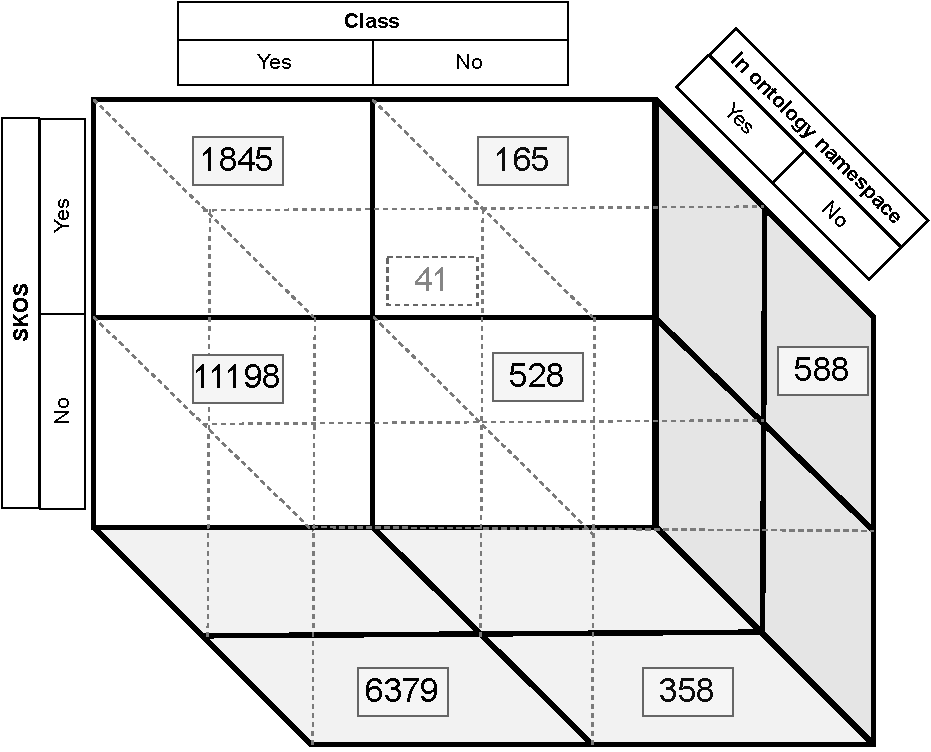
\includegraphics[width=8cm]{figures/cube-aggregation.pdf}
    \caption{Aggregation of instances in three analytical dimensions}
    \label{fig:cube-aggregation}
\end{figure}
